\documentclass[11pt]{report}

\usepackage[a4paper,margin=1in]{geometry}
\usepackage[utf8]{inputenc}
\usepackage{titlesec}
\usepackage[T1]{fontenc}
\usepackage{float}
\usepackage{graphicx}
\usepackage{paralist}
\usepackage{multicol}
\usepackage{tikz}
\usepackage{tabularx}
\usepackage{adjustbox}
\usepackage[acronym,toc,nonumberlist,nogroupskip]{glossaries}
\usepackage{enumitem}
\usepackage{xltabular}
\usepackage{dirtree}
\usepackage{minted}


% setup bibliography
\usepackage[style=ieee]{biblatex}
\addbibresource{references.bib}

% setup hyperlinks
\usepackage{hyperref}
\hypersetup{
    colorlinks=true,
    citecolor=black,
}

% setup debug box command for places things are missing
\newcommand{\todo}[1]{\fbox{\parbox{\textwidth}{\textbf{TO-DO:} #1}}}

% Glossary entry
\makenoidxglossaries

\newglossaryentry{ppu_g}{
    name={Picture Processing Unit},
    description={The part of the Gameboy that is responsible for rendering the game}
}
\newglossaryentry{ppu}{
    type=\acronymtype,
    name={PPU},
    description={Picture Processing Unit},
    first={Picture Processing Unit (PPU)\glsadd{ppu_g}},
}

\newglossaryentry{gb}{
    type=\acronymtype,
    name=GB,
    description={Gameboy},
    first={Gameboy (GB)}
}

\newglossaryentry{gbc}{
    type=\acronymtype,
    name=GBC,
    description={Gameboy Color},
    first={Gameboy Color (GBC)}
}

\newglossaryentry{os}{
	type=\acronymtype,
	name=OS,
	description={Operating System},
	first={Operating System (OS)}
}

\newglossaryentry{cpu}{
    type=\acronymtype,
    name=CPU,
    description={Central Processing Unit},
    first={Central Processing Unit (CPU)}
}

\newglossaryentry{apu_g}{
    name={Audio Processing Unit},
    description={The part of the Gameboy that is responsible with processing the game's audio}
}

\newglossaryentry{apu}{
    type=\acronymtype,
    name=APU,
    description={Audio Processing Unit},
    first={Audio Processing Unit (APU)}
}

\newglossaryentry{rom}{
    type=\acronymtype,
    name={ROM},
    plural={ROMs},
    description={Read-Only Memory},
    first={Read-Only Memory (ROM)},
    firstplural={Read-Only Memory (ROM)}
}

\newglossaryentry{mbc}{
    type=\acronymtype,
    name={MBC},
    plural={MBCs},
    description={Memory Bank Controller},
    first={Memory Bank Controller (MBC)},
    firstplural={Memory Bank Controllers (MBCs)}
}

\newglossaryentry{oam}{
    type=\acronymtype,
    name={OAM},
    description={Object Attribute Memory},
    first={Object Attribute Memory (OAM)},
}

\newglossaryentry{dma}{
    type=\acronymtype,
    name={DMA},
    description={Direct Memory Access},
    first={Direct Memory Access (DMA)},
}

\newglossaryentry{dmg_g}{
    name={Dot Matrix Game},
    description={The model name of the Gameboy. It is often used to refer to the "base" Gameboy (in contrast with GBC for the Gameboy Color)}
}
\newglossaryentry{dmg}{
    type=\acronymtype,
    name={DMG},
    description={Dot Matrix Game},
    first={Dot Matrix Game (DMG)\glsadd{dmg_g}},
}

\newglossaryentry{tcyc}{
    name={T-Cycle},
    description={A T-cycle is the smallest step the internal clock of the Gameboy can do. This means the rate of T-cycle is that of the CPU, ie. 4.19Mhz}
}

\newglossaryentry{mcyc}{
    name={M-Cycle},
    description={An M-Cycle (or machine cycle) is the smallest step the CPU of the Gameboy can do. Because all instructions of the CPU are multiples of 4, instruction lengths and timings are usually referred to in M-cycles (e.g. \texttt{LD A, B} takes 4 T-cycles, thus 1 M-cycle)}
}

\newglossaryentry{mmap}{
    name={Memory Map},
    description={The memory map is what determines where each address leads to - it can be seen as a list of non-overlapping ranges}
}

\newglossaryentry{msb}{
    type=\acronymtype,
    name={MSB},
    description={Most Significant Bits},
    first={Most Significant Bits (MSB)},
}

% setup paragraph spacing
\setlength{\parskip}{\baselineskip}
\setlength{\parindent}{0pt}
\titlespacing\section{0pt}{12pt plus 4pt minus 2pt}{-8pt}\relax
\titlespacing\subsection{0pt}{12pt plus 4pt minus 2pt}{-10pt}\relax
\titlespacing\subsubsection{0pt}{12pt plus 4pt minus 2pt}{-10pt}\relax

\begin{document}

% setup fonts

\begin{titlepage}
    \begin{center}
        \vspace*{1cm}

        \Huge
        \textbf{Emmy: The Gameboy Color Emulator}\\
        6CCS3PRJ Final Project

        \vspace{1.5cm}
        \Large
        Classic video game console emulation

        \vfill

        Author: Oscar Sjöstedt\\
        Student ID: K20040078\\
        Supervisor: Ian Kenny

        \vspace{1.5cm}

        \Large
        Draft Two \\
        \today \\
        King's College London \\

    \end{center}
\end{titlepage}

\null\vfill

\begin{abstract}
    This project aims to create a Gameboy emulator web-application, in other words a program capable of receiving Gameboy game files (commonly refered to as ROMs), and interpreting such ROM to play the game (or execute the program) it contains. The emulator will be usable in browsers, for both desktop computers and mobile devices that may not have access to a physical keyboard. The emulator will also contain debugging capacities, to allow other emulator developers to use it when comparing with their emulator and working on it.

    The objective of this project is to create a piece of software that could be used by anyone wanting to emulate retro games, without the need for any technical knowledge on emulators or downloading anything (except the ROMs that need to be obtained separately).
\end{abstract}
\vfill

\clearpage

{\hypersetup{hidelinks}\tableofcontents} 

\clearpage

\chapter{Background}

\section{Emulation}

An emulator is ``hardware or software that permits programs written for one computer to be run on another computer'' \cite{emulator_def}. The imitated computer is the \textit{guest}, and the one that imitates is the \textit{host}. Emulators are nowadays mainly found in the form of software, and have many different uses, from preservation to hardware development.

Emulation was technically born with the first computers: the very first computer, the Colossus made in 1941, was built to imitate the Enigma machine \cite{emulator_origin}. However emulation was properly studied towards the end of the twe ntieth century, when computing power started to steadily increase. One of the earliest instances of emulation as an actual feature is with the IBM System/360. This computer supported emulation of previous models, such as the IBM 709, 7090, 7094 and 7094 II \cite{ibm_emulation}.

Nowadays emulation is used when researching and creating new hardware - using virtual systems to design a system and look for errors is much more cost-effective \cite{emu_in_design}. The real system doesn't have to actually be produced, and if something goes wrong it is very simple to look for the error in the simulated system, through logging or stepping through the simulation.

Emulation is also vital for preservation: as transistors and motherboards age, old systems become unusable, and with them the software they ran. Emulating these systems is often the only future-proof and sustainable way to keep this software usable.

Finally, another common use for emulation is virtual machines. These programs allow running another \gls{os} on a computer, which can be used for instance when developing for other systems, without needing to use the physical device directly, for instance when developing a Windows-compatible app with a Linux computer.

\section{Video Game Emulation}

Video game emulation is the art of emulation applied to video game hardware systems. This allows the host to run games destined for the original console. This usually requires precise understanding of the console's hardware and functioning, as games may rely on specific behaviours and edge cases to function. This task is rendered harder by the fact that often game consoles are poorly documented, as they are proprietary hardware and programmer guides written for them cannot be legally distributed.

Video game emulation started in the 90s when computers were powerful enough to properly simulate console systems. Although precise dates are hard to get, the first console emulators seem to be either from 1990 or 1993 \cite{first_nes_emu}, and were able to run some NES games. The first Gameboy emulators were in the late 90s, with the \href{http://fms.komkon.org/VGB/}{Virtual GameBoy} in 1995 and \href{https://problemkaputt.de/gmb.htm}{NO\$GMB} in 1997 (although it's \href{https://problemkaputt.de/gmbhist.htm}{history page} seems to indicate development started in 1993) \cite{first_gb_emus}.

The original game files and assembled code for video games is copyrighted material, and is referred to as the \gls{rom} of the game. Although distributing these \glspl{rom} is usually illegal, there also exist copyright free \glspl{rom}: games created by developers that chose to license them under Creative Commons licenses, for instance. Websites such as \href{https://www.retroveteran.com/category/nintendo-game-boy-color/}{Retro Veteran} host wide collections of legal \glspl{rom}.

\section{Gameboy, Gameboy Color}

The \gls{gb} is an 8-bit handheld video game console, released in 1989. It has a small $160 \times 144$ pixel screen, and has a Sharp LR35902 as its \gls{cpu}, clocked at 4.19MHz. In 1998, the \gls{gbc} was then released. Seen as the successor of the \gls{gb}, it contains a screen of the same resolution, but supporting colors, from a palette of 32768 colors. It contains the same \gls{cpu} as its predecessor, a Sharp LR35902, with now two modes: a 4.19MHz mode and a 8.38MHz mode (double-speed mode). This allows the \gls{gbc} to be backwards compatible with most \gls{gb} games - there are a few exceptions to this, games that used hardware bugs of the original \gls{gb} that were fixed in the \gls{gbc}.

From an emulation perspective, the \glsdesc{gbc} can thus be seen as an extension of the Game Boy - it has an identical CPU (although with a toggle-able double speed mode), and most of the memory layout is identical. To keep the remaining of this document simple, if not stated, "GB" will refer to both the original \glsdesc{gb} and the \glsdesc{gbc}, as they are very similar. \gls{dmg} refers to the original \glsdesc{gb} model.

\section{Existing Literature}

\subsection{Gameboy Documentation}

The \glsdesc{gb} is one of the best documented consoles for emulation, and an array of resources exist to get started writing a new one. Some of the resources I used to write my emulator are:

\begin{compactitem}
    \item \href{https://gbdev.io/pandocs/}{Pandocs} is a technical reference of how the \gls{gb} works. It is extremely complete and covers a wide range of topics, so it is useful to get a global view of a problem. It is one of the most referenced pieces of literature on the console.
    \item \href{https://meganesu.github.io/generate-gb-opcodes/}{GB CPU Instructions} is a table containing all instructions the \gls{gb} \gls{cpu} has, as well as information on the amount of cycles taken by the instruction, the bytes of memory used, the flags affected by the operation, and a description of the instruction.
    \item \href{https://gekkio.fi/files/gb-docs/gbctr.pdf}{GBCTR} (Gameboy Complete Technical Reference) is an unfinished document that contains very detailed information on the \gls{cpu} and other components of the \gls{gb}. Although incomplete, it provides a much lower-level view of the details of the \gls{gb} (compared to Pandocs), making it useful to emulate very specific behaviour.
    \item \href{https://gbdev.gg8.se/wiki/}{GB dev wiki} is a wiki containing additional information on the \gls{gb}, including guides to making games and explanations on some hardware quirks.
\end{compactitem}

\subsection{Existing Emulators}

Furthermore, to aid with developing the emulator, I sometimes had to look through the open source code of existing emulators, to understand how they implemented certain things. These projects include:

\begin{compactitem}
    \item \href{https://github.com/mattbruv/Gameboy-Crust}{Game Boy Crust} is a simple \gls{gb} emulator written in Rust. It is quite incomplete but has a comprehensive structure, so it's a good project to first figure out how emulators work.
    \item \href{https://github.com/Atem2069/accurateboy}{AccurateBoy} is a highly accurate emulator, in particular for its \gls{ppu} that has pixel-perfect accuracy.
    \item \href{https://github.com/samcday/oxideboy}{oxideboy} is another \gls{gb} emulator written in Rust, that is much more complete and helpful for some edge cases.
    \item \href{https://github.com/LIJI32/SameBoy}{SameBoy} is one of the most accurate open source \gls{gb} and \gls{gbc} emulators, written in C. It is much more technically complex but still useful to understand edge cases, especially since it is the emulator I use and compare mine with.
    \item \href{https://github.com/Gekkio/mooneye-gb}{Mooneye GB} is a \gls{gb} research emulator written in Rust. It passes most of the Mooneye test ROMs, making it helpful when encountering issues with these tests.
    \item \href{https://github.com/taisel/GameBoy-Online/}{GameBoy-Online} is a high-accuracy JavaScript emulator, that I used when unsure on how to interface the emulator with the browser (notably for the \gls{apu}).
    \item \href{https://github.com/juchi/gameboy.js/}{Gameboy.js} is another JavaScript emulator. It is fairly simply and inaccurate, but is easily hackable. As such it's the emulator I used when starting the emulator, to compare mine with.
    \item \href{https://github.com/mvdnes/rboy}{rboy} is an emulator written in Rust, that I used when developing the \gls{apu} to compare mine with, as it passes some test \glspl{rom} I struggled with.
\end{compactitem}

\subsection{Gameboy Test ROMs}
\label{sec:gb-test-roms}

Finally, some of the most helpful resources I've used are test \glspl{rom}, that can be run on an emulator and output if the emulator passes certain tests (these can be \gls{cpu}, \gls{ppu}, timer tests, etc.). They help quickly diagnose issues, and also allow me to mark certain components and parts of the emulator as "complete", meaning I can rely on these components and know they are fully-functional. These test \glspl{rom} also have the advantage of being open source, meaning I can understand what the test does, and if it fails figure out where and why it goes wrong without having to decompile the \gls{rom}.

An other advantage to using test \gls{rom} is that they re-use the same framework across a given suite to report results. This means the result of the test is usually logged somewhere in the console, and testing can easily be automated without having to compare the displayed image.

The test \glspl{rom} I used are:

\begin{compactitem}
    \item \href{https://github.com/retrio/gb-test-roms/}{Blaarg test \glspl{rom}} are some of the most well-known and used \gls{gb} test \glspl{rom}. They include tests for the \gls{cpu}, the timings of instructions, and some other functionality.
    \item \href{https://github.com/Gekkio/mooneye-test-suite}{Mooneye test \glspl{rom}} is a much more complete and tougher test suite, that verifies most components of the \gls{gb}: \gls{cpu} instructions, memory timings of specific instructions, behaviour of \glspl{mbc}, timing of the \gls{oam} \gls{dma}, \gls{ppu} timings, timer timings, etc.
    \item Acid Test (\href{https://github.com/mattcurrie/dmg-acid2}{\gls{dmg}}, \href{https://github.com/mattcurrie/cgb-acid2}{\gls{gbc}}) is a test that verifies the \gls{ppu} of the \gls{gb} displays data properly (to line-rendering accuracy), for both \glsdesc{gb} and \glsdesc{gbc} displays.
    \item \href{https://github.com/LIJI32/SameSuite/}{SameSuite} is a test suite that is valuable for its \gls{apu} tests: it uses the PCM12 and PCM34 registers exclusive to the \gls{gbc} to inspect the exact ouput of the \gls{apu} (whereas other test \glspl{rom} tend to inspect the on/off status of the channels, which is much less accurate).
\end{compactitem}

\chapter{Requirements and Specification}

\section{Requirements}

\subsection{User Requirements}

\begin{enumerate}[start=1,label=U\arabic*.]
    \item Run \glsdesc{gb} games to a satisfiable fidelity, with proper rendering and controls emulation.
    \item Run \glsdesc{gbc} games to a satisfiable fidelity, with proper rendering and controls emulation.
    \item Allow the user to run \gls{gb} and \gls{gbc} games for both a \glsdesc{gb} and a \glsdesc{gbc} (ie. allow using a \gls{gbc} for a \texttt{.gbc} file, and a \gls{gb} for a \texttt{.gb} file).
    \item Allow the user to save the state of the game, to continue their playthrough later. The state can simply be saved as a downloaded file, and re-uploaded later to continue the game.
    \item Allow the user to change the speed at which the game is played: double speed mode, half speed mode, etc.
    \item Have some debug functionality, to inspect the state of the console at any given time.
    \item Allow users to pause the console, and add breakpoints to stop execution at specific moments.
    \item Allow the user to switch between rendering modes (nearest-neighbour, LCD display, scale2, etc.)
    \item Allow the user to switch the colour palette of the \gls{dmg} emulation.
\end{enumerate}

\subsection{System Requirements}

\begin{enumerate}[start=1,label=F\arabic*.]
    \item The system can receive a \gls{rom} file, construct an instance of the emulated console, and run the code inside said \gls{rom}.
    \item The system emulates different components of the \gls{gb} and \gls{gbc}, with as much precision as possible (\gls{mcyc} precision).
    \item The system renders the output of the emulator to a Web \texttt{<canvas />}.
    \item The system creates the required DOM elements for the web-app, and updates them as needed.
    \item The system listens to key presses and releases to emulate controls through the keyboard.
    \item For touch devices, the system may render buttons to simulate the console's controls.
\end{enumerate}

\subsection{Non-Functional Requirements}

\begin{enumerate}[start=1,label=N\arabic*.]
    \item The emulator should be accessible on computers through a web browser equipped with a recent version of JavaScript.
    \item The emulator should be accessible on mobile devices through a web browser equipped with a recent version of JavaScript.
    \item The emulator should be accessible on computers through a standalone app.
    \item Maximise the tests passed by the emulator (see \nameref{sec:gb-test-roms})
    \item Have the code be well documented, allowing new-comers to the project and to \gls{gb} emulation to easily understand what is going on - if possible with links to relevant \glsdesc{gb} emulation resources.
\end{enumerate}


\section{Specification}


\begin{xltabular}{\textwidth}{|c|X|c|}
    \hline
    \textbf{Code} & \textbf{Specification} & \textbf{Importance}\\
    \hline\hline
    \endhead

    U1 & User can upload a \gls{gb} \gls{rom} file (\texttt{.gb}), and the emulator will run the game. The keyboard can be used to control the game, and the output is displayed. & High \\ \hline
    U2 & User can upload a \gls{gbc} \gls{rom} file (\texttt{.gbc}), and the emulator will run the game. The keyboard can be used to control the game, and the output is displayed. & Medium \\ \hline
    U3 & User can upload a \gls{gb} \gls{rom} file (\texttt{.gb}). The user can switch between a \gls{dmg} and a \gls{gbc} emulator. & Medium \\ \hline
    U4 & User can press a button to download a save of their game (or, alternatively, the save can be stored inside the browser with a technology like \href{https://developer.mozilla.org/en-US/docs/Web/API/IndexedDB_API}{IndexedDB}) & Low \\ \hline
    U5 & User can select the speed of emulation, to dynamically accelerate/decelerate the game. & Medium \\ \hline
    U6 & User can see debug information of the emulator. This information includes the current tileset, background map, time to draw a frame, and register information. & Low \\ \hline
    U7 & User can pause the console emulation through a button. They can also input conditions for which the console should break execution. & Low \\ \hline
    U8 & User can dynamically switch the rendering filter via a dropdown button. & Low \\ \hline
    U9 & User can dynamically switch the colour palette of the GameBoy via a dropdown button. & Low \\ \hline

    F1 & A \gls{rom} file can be uploaded, is transformed into an \texttt{UInt8Array} (because the \gls{gb} is an 8-bit system), and the appropriate object is created to run the code. & High \\ \hline
    F2 & Different components exists as different classes, respecting typical OOP principles such as encapsulation and inheritance when relevant. & High \\ \hline
    F3 & A \texttt{<canvas />} element is created, and is updated with the output of the emulator after every frame is drawn (ie. at the start of each VBlank mode). & High \\ \hline
    F4 & The \href{https://preactjs.com/}{Preact} framework is used to handle the UI of the web-app. & High \\ \hline
    F5 & Listeners are added to the environment's \texttt{window} to listen to all key presses and releases. The emulator can then request for a control update, by reading the state of keys. & High \\ \hline
    F6 & If a touch device is detected, button are added to the UI and are used by the emulator as inputs. & Medium \\ \hline

    N1 & A deployed version of the web-app is accessible on a desktop browser and provides full functionality, via keyboard and mouse inputs. & High \\ \hline
    N2 & A deployed version of the web-app is accessible on a mobile device browser and provides full functionality, via touch controls. & Medium \\ \hline
    N3 & A downloadable version of the web-app can be used on a computer and provides full functionality, via keyboard and mouse inputs. & Low \\ \hline
    N4 & As many possible tests as possible should be passed, while ensuring previously passing tests don't start failing. & Medium \\ \hline
    N5 & Main methods and variables must be properly documented, and have links to appropriate online resources to documentation about said element. & High \\ \hline
\end{xltabular}

\chapter{Design}

The project uses \href{https://preactjs.com/}{Preact}, a light-weight alternative to the more popular \href{https://reactjs.org/}{React} framework. I chose to use Preact because the front-end of the web-app is extremely light weight, so I wanted to avoid bloating the app with a heavy framework such as React. The React framework once GZipped and minified is around 31.8Kb, when Preact is only 4Kb (87\% less).

The language used for the project is \href{https://www.typescriptlang.org/}{TypeScript}, a typed version of JavaScript. This will prove very useful as the project gets larger, to ensure the correctness of code.

The project is divided in two parts:
\begin{compactitem}
    \item The root directory contains the UI for the web-app. Most of the code is in \texttt{app.tsx}, since the front-end is quite light-weight (a few buttons, a file input, and the logic to create the emulator as well as handling inputs and outputs).
    \item  The \texttt{emulator/} directory contains the actual \gls{gb} emulator. Although most classes and interfaces used are exported, only three elements are needed to properly interact with the emulator:
    \begin{compactitem}
        \item \texttt{GameBoyColor.ts} handles the core loop of the system: it ticks both the \gls{cpu} and the rest of the system, bundled under the class \texttt{System}.
        \item \texttt{GameBoyOutput.ts} is a simple interface, with optional methods to receive any output produced by the emulator (see figure \ref{fig:gameboyoutput})
        \item \texttt{GameBoyInput.ts} is a simple interface with a required \texttt{read()} method that should return an object with the current inputs for the console (see figure \ref{fig:gameboyinput}).
    \end{compactitem}
\end{compactitem}

\begin{figure}[h]
    \begin{minted}{typescript}
interface GameBoyOutput {
    receive?(data: Uint32Array): void;
    debugBackground?(data: Uint32Array): void;
    debugTileset?(data: Uint32Array): void;
    serialOut?(data: number): void;
    errorOut?(error: unknown): void;
    stepCount?(steps: number): void;
    cyclesPerSec?(cycles: number): void;
    frameDrawDuration?(ms: number): void;
}
    \end{minted}
    \caption{\texttt{GameBoyOutput} interface methods}
    \label{fig:gameboyoutput}
\end{figure}

\begin{figure}[h]
    \begin{minted}{typescript}
type GameBoyInputRead = {
    up: boolean;
    down: boolean;
    left: boolean;
    right: boolean;

    a: boolean;
    b: boolean;
    start: boolean;
    select: boolean;
};

interface GameBoyInput {
    read(): GameBoyInputRead;
}
    \end{minted}
    \caption{\texttt{GameBoyInput} interface method}
    \label{fig:gameboyinput}
\end{figure}

\section{Emulator Frontend}

The frontend of the emulator is written in Preact, allowing us to create a simple, fast and lightweight UI to control it. It contains the emulator title, the control buttons, some debug information, and the emulator video output (see figure~\ref{fig:emmy-home}).

The main controls for the emulator are the 6 buttons above the screen. These are, from left to right:
\begin{compactitem}
    \item Pause/play: pauses or starts the emulator.
    \item Step one \gls{mcyc}: this is particularly useful when debugging to figure out exactly when something goes wrong. It is only enabled when the emulator is paused.
    \item Debug view: displays the tileset and background map alongside the executing game (see figure~\ref{fig:emmy-debug-view})
    \item Compare mode: runs a second open-source emulator (\href{https://github.com/juchi/gameboy.js/}{Gameboy.js}) at the same time as my emulator. This is useful to compare graphics and check it works somewhat properly.
    \item Test mode: stops execution of the current game, and instead runs a series of tests automatically, recording which ones pass and fail. The result of the tests is logged to the console as a table, allowing to quickly check to what is and isn't working (see figure~\ref{fig:emmy-test-output}). The state of a test can be: a green check (passed), a red cross (failed), a headstone (failed due to error) or an hourglass (failed due to timeout).
    \item Speed-boost toggle: a toggle button that speeds up the emulator to triple its base speed.
\end{compactitem}

Further more the emulator currently displays some debug data, to check the performance of it. From top to bottom, these are:
\begin{compactitem}
    \item The total number of instructions executed so far.
    \item The number of \glspl{tcyc} executed per second - this is to compare with the ideal of 4.19MHz.
    \item The number of milliseconds needed to render a frame. The \gls{gb} renders at 60 frames per second (60Hz), so this measures the time taken to perform $(4.19*10^6)/60\approx 69000$ \glspl{tcyc}.
\end{compactitem}

\begin{figure}[h]
    \centering
    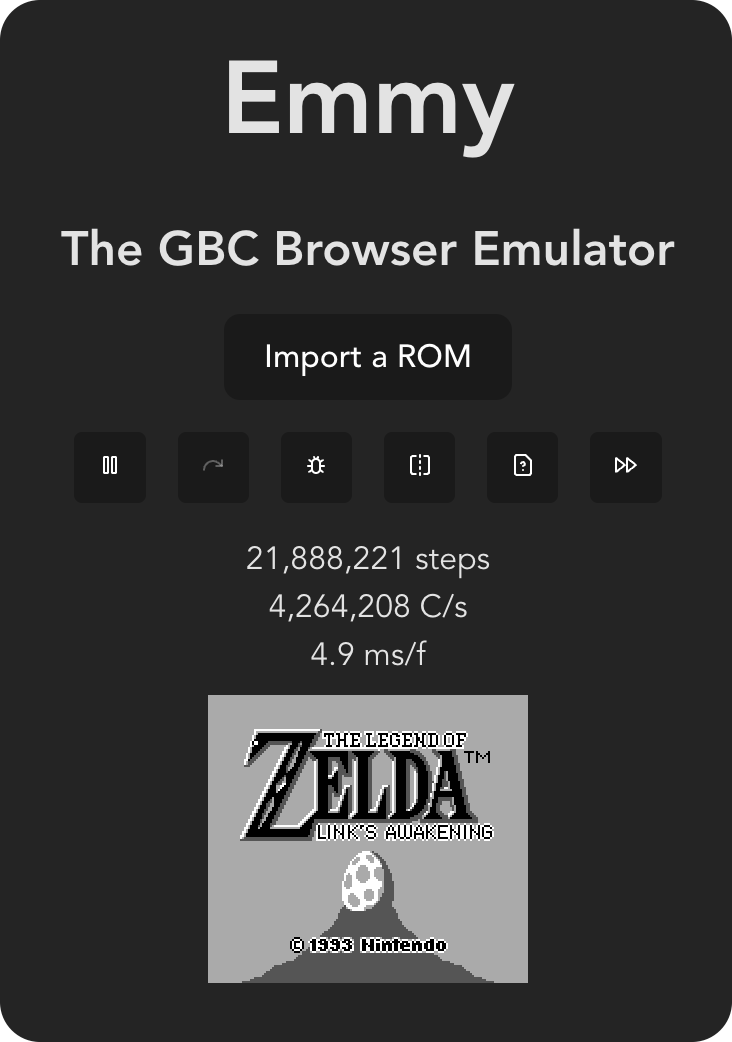
\includegraphics[width=5cm]{images/emmy-home-page.png}\\
    \caption{Home page of the emulator}
    \label{fig:emmy-home}
\end{figure}

\begin{figure}[h]
    \centering
    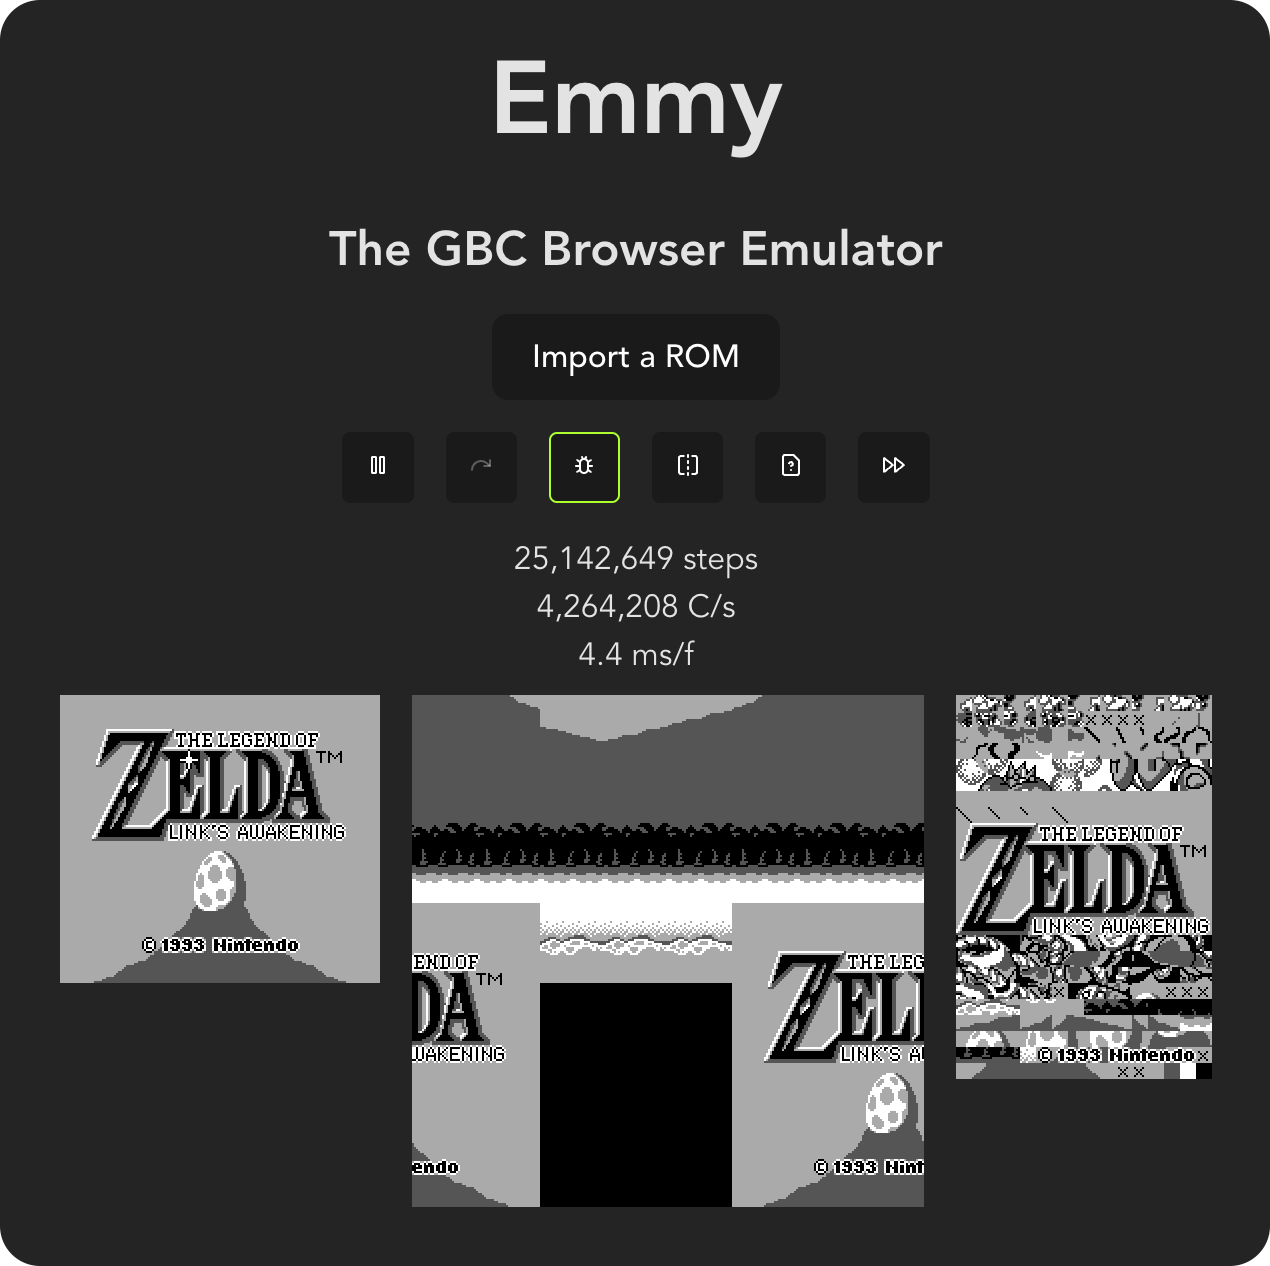
\includegraphics[width=8cm]{images/emmy-debug-view.png}\\
    \caption{Debug view of the emulator}
    \label{fig:emmy-debug-view}
\end{figure}

\begin{figure}[h]
    \centering
    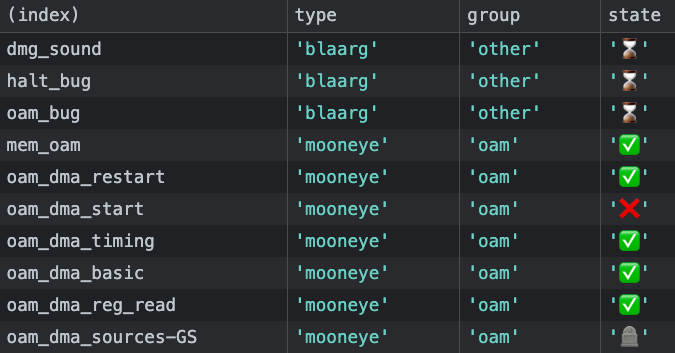
\includegraphics[width=8cm]{images/emmy-test-output.png}\\
    \caption{Snippet of test mode output}
    \label{fig:emmy-test-output}
\end{figure}

\section{Emulator Backend}

To keep the logic of the hardware, divided in different components, the structure of the emulator has a similar format, with different classes implementing the behaviour of the different parts of the \glsdesc{gb}.

\subsection{Addressable}

The \texttt{Addressable} interface is implemented by most classes of the emulator: \texttt{System}, \texttt{Register}, \texttt{MBC}, etc. It is simple, and provides a read and a write method (see figure \ref{fig:addressable}). The advantage of using it is that when implementing adressing logic with large switch-statements I can simply return any type of components that adheres to the interface, and the receiving method is agnostic of if it's dealing with a register, memory, or a component.

\begin{figure}[h]
    \begin{minted}{typescript}
interface Addressable {
    read(pos: number): number;
    write(pos: number, data: number): void;
}
    \end{minted}
    \caption{\texttt{Addressable} interface method}
    \label{fig:addressable}
\end{figure}

\subsection{System}

The \texttt{System} class implements the motherboard, and the general connection between elements. It handles the ticking of the \gls{ppu}, timer and \gls{oam} \gls{dma}. Furthermore, it is the component that links all of the data together: whenever a component is ticked (any of the above or the \gls{cpu}), the \texttt{System} instance is passed, so that the components can read and write to the rest of the system. It does implement \texttt{Addressable}, and internally has a \texttt{getAdress} method that returns both an \texttt{Addressable} and a number (the index to read or write to). This way the addressing logic to determine what component is accessed depending on the address isn't duplicated.

\subsubsection{\texttt{getAddress} optimisation}

Because \texttt{System} is a higly used component and is accessed for almost every read and write, the \texttt{getAddress} method is under a lot of pressure. As such, it was the source of a major re-write during development, which improved performances significantly.

Initially it was implemented as a list of if-statements for different ranges of the \gls{mmap}, as well as an object where the keys were different register-addresses. The code would first check if the key exists in the register object (it thus served as a map), and if not it would then go through a series of if-conditions (see figure \ref{fig:getaddress-before}).

This proved quite costly, for three main reasons:
\begin{compactitem}
    \item This code creates a new object every time it is called, when checking for the registers' addresses.
    \item The if-conditions for the ranges of the biggest areas of memory (everything between \texttt{0x0000} and \texttt{0xffef}) happened after the register checks, which delayed response for these reads and writes.
    \item Chaining if-conditions is unneficient, as the JS engine must step through all conditions and check the values each time. Furthermore, although having both the lower and upper bound of the memory section indicated in the condition (e.g. \texttt{0x0000 <= pos \&\& pos <= 0x7fff} for $[\texttt{0x0000}; \texttt{0x7fff}]$) makes the translation from \gls{mmap} to code easier, it is slower, since only the upper bound of the range is needed for the condition \textit{if} all the ranges below have already returned.
\end{compactitem}

My intial optimisation - and the one that had the most impact on this method - was fixing the last two points: removing these if-conditions, and moving these areas higher in the code.

The way the addressing circuitry works is that addresses are not compared in their entirety: the circuit checks for small sections of the address, and then maps those to more precise locations. As such the main areas of memory can usually be identified by their \gls{msb} - usually the most significant nybble (see figure \ref{fig:memory-map-largest}).

\begin{figure}[h]
    \centering
    \begin{tabular}{|l|l|l|}
    \hline
    \textbf{Start} & \textbf{End} & \textbf{Description} \\ \hline
    0000 & 3FFF & 16 KiB ROM bank 00 \\ \hline
    4000 & 7FFF & 16 KiB ROM Bank 01$\sim$NN \\ \hline
    8000 & 9FFF & 8 KiB Video RAM (VRAM) \\ \hline
    A000 & BFFF & 8 KiB External RAM \\ \hline
    C000 & CFFF & 4 KiB Work RAM (WRAM) \\ \hline
    D000 & DFFF & 4 KiB Work RAM (WRAM) \\ \hline
    \end{tabular}\\
    Source: \href{https://gbdev.io/pandocs/Memory_Map.html}{Pandocs}
    \caption{Memory map for the largest chunks of memory}
    \label{fig:memory-map-largest}
\end{figure}

This means that for this area of memory we can simply isolate the last nybble, and then create a switch-statement over it to map directly to specific areas. This removes the need for the if-conditions, and is also faster as it is evaluated much earlier on (see figure \ref{fig:getaddress-after}).

I then ran a simple test to verify the performance improvement. I ran the first 25 million instructions of the \href{https://github.com/retrio/gb-test-roms/tree/master/cpu_instrs}{\texttt{cpu\_instrs}} test \gls{rom} - I chose this sample because it is considerably large, because the test itself requires around 25 million instructions to complete, and because this test checks for all instructions of the \gls{cpu}, meaning that it exercices most configurations of the \gls{cpu} and system. For the measurement, I used \texttt{window.performance.now()} before and after each drawn frame, and summed the values.

The result was the following: $33 955.9$ms before the change, and $20 039.1$ after the change. The relative difference is thus $\frac{20 039.1-33 955.9}{33 955.9}=-0.4098$, thus reducing time taken by $40.98\%$.

Note that, although this may vary based on engine, switch statements aren't faster than if-conditions in JavaScript. \href{https://jsbench.me/qqlbqix93t/1}{This simple test-suite} has a switch statement with 16 cases, along with an object with 16 keys and an if-statement with 16 clauses. On my browser (Google Chrome v108), the switch-statement proved the fastest, with the switch and if statements lagging behind by being respectively $69.81\%$ and $70.23\%$ slower. As such I suspect this improvement to be mainly due to the switch statement being moved at the beginning of the function, thus skipping the more expensive object creation.

This also means that improvements to this method can still be done. Using the "Performance" tab of Chrome Developer Tools, I measured the performance of the whole emulator when running the first 10 million instructions of this same test. The results I got indicated that \texttt{getAddress} is still the third method with the higest \textbf{self-time} (see figures \ref{fig:performance-getaddress-before} and \ref{fig:performance-getaddress-after}). Here self-time refers to the time taken inside the method itself, and total time is the time taken by the method and the methods it calls. Note how \texttt{getAddress} still has the third highest self-time, meaning that the content of the method itself takes time (although this value dropped from $40.7\%$ to $7.7\%$). The increase is self-time percentage (not time!) for all other methods is simply due to the fact that by making \texttt{getAddress} faster the self-time of these other methods (that all call \texttt{getAddress}) gets proportionally higher compared to their total time.

\begin{figure}[h]
    \centering
    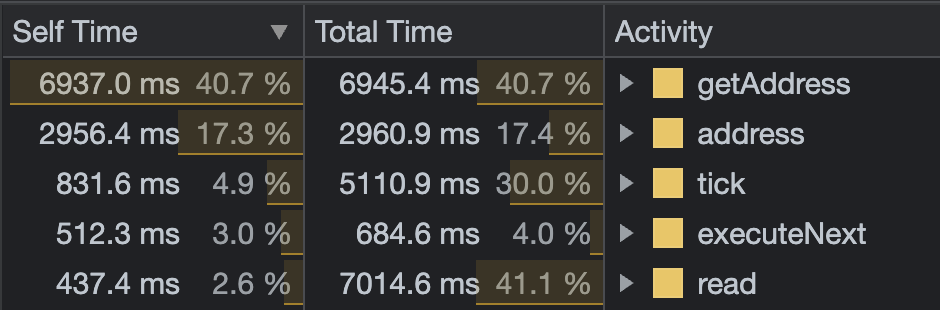
\includegraphics[width=8cm]{images/get-address-before.png}\\
    \caption{Performance measurement of the emulator before \texttt{getAddress} optimisation}
    \label{fig:performance-getaddress-before}
\end{figure}

\begin{figure}[h]
    \centering
    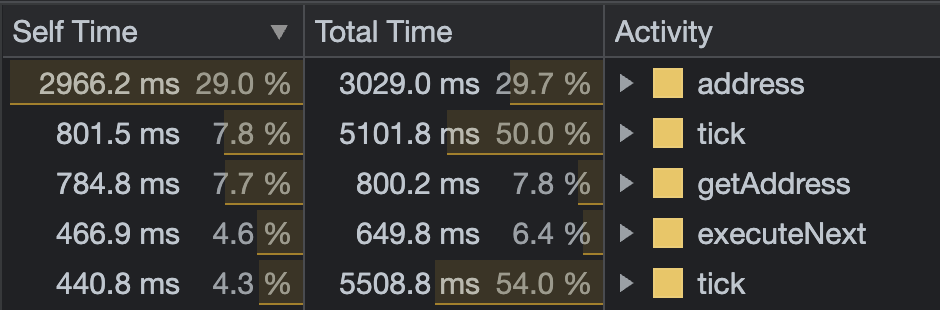
\includegraphics[width=8cm]{images/get-address-after.png}\\
    \caption{Performance measurement of the emulator after \texttt{getAddress} optimisation}
    \label{fig:performance-getaddress-after}
\end{figure}

\begin{figure}[h]
    \begin{minted}{typescript}
protected getAddress(pos: number): AddressData {
    if (pos < 0x0000 || pos > 0xffff)
        throw new Error(`Invalid address to read from ${pos.toString(16)}`);

    const register = {
        0xff00: this.joypad,
        ...
        0xffff: this.intEnable,
    }[pos];
    if (register !== undefined) return [register, pos];

    if (0x0000 <= pos && pos <= 0x7fff) return [this.rom, pos]; // ROM Bank
    ...
    if (0xfe00 <= pos && pos <= 0xfe9f) return [this.oam, pos]; // OAM

    // Unmapped area, return 'fake' register
    return [{ read: () => 0xff, write: () => {} }, 0];
}
    \end{minted}
    \caption{Initial implementation of \texttt{getAddress}}
    \label{fig:getaddress-before}
\end{figure}

\begin{figure}[h]
    \begin{minted}{typescript}
protected getAddress(pos: number): AddressData {
    if (pos < 0x0000 || pos > 0xffff)
        throw new Error(`Invalid address to read from ${pos.toString(16)}`);

    switch ((pos >> 12) as Int4) {
        case 0x0:
            return [this.rom, pos]; // ROM
        ...
        case 0xe:
            return [this.wram, pos & (WRAM_SIZE - 1)]; // ECHO RAM
        case 0xf:
            break; // fall through - ECHO RAM + registers
    }

    const register = {
        0xff00: this.joypad,
        ...
        0xffff: this.intEnable,
    }[pos];
    ... rest is unchanged
}
    \end{minted}
    \caption{Optimised implementation of \texttt{getAddress}}
    \label{fig:getaddress-after}
\end{figure}

\clearpage
\subsection{CPU}

The \gls{cpu} is the most important part of the emulator, and allows running the code from the \gls{rom} by reading the operation code (or opcode) and executing the matching action.

\subsubsection{Initial Instruction Set}

Because the \glsdesc{gb} is an 8-bit system, opcodes are 8 bits (or one byte) long, giving in theory a maximum of $2^8=256$ operations. However in the \gls{gb} the operation \texttt{0xCB} gives access to an extended instruction set, meaning that when reading \texttt{0xCB} the \gls{cpu} will read the next byte and use a different logic to execute the operation. This means there are now $2^8 - 1 + 2^8=511$ operations. The \gls{gb} also has 11 forbidden opcodes (the console will lock itself if they are executed), meaning there are in total $2^8 - 12 + 2^8 = 500$ operations to implement.

Multiple techniques exist to handle this large number of operations:

\begin{compactitem}
    \item Have a large switch-statement for all operations
    \item Have a map, that maps an opcode to a function to execute
    \item Decode the operation by reading specific parts of the byte, and generate the instructions dynamically
\end{compactitem}

I initially had a large object, with all the opcodes as keys, that would then contains a simple function that returns the number of cycles taken by the instruction (see figure \ref{fig:instset-first}). This however proved quite repetitive and prone to errors. Furthermore, this wasn't \gls{mcyc} accurate: the \gls{cpu} instruction was executed as one monolithic block, when in reality all reads and writes are executed at a separate \gls{mcyc} - this becomes very important when the timer, \gls{oam} and \gls{ppu} are involved, as they run in parallel with the \gls{cpu}, so memory accesses to these components may return different values depending on the \gls{mcyc}.

\begin{figure}[h]
    \begin{minted}{typescript}
protected instructionSet: Partial<Record<number, InstructionObject>> = {
    // NOP
    0x00: () => 1,
    // LD BC/DE/HL/SP, d16
    0x01: (s) => { this.regBC.set(this.nextWord(s)); return 3; },
    0x11: (s) => { this.regDE.set(this.nextWord(s)); return 3; },
    0x21: (s) => { this.regHL.set(this.nextWord(s)); return 3; },
    0x31: (s) => { this.regSP.set(this.nextWord(s)); return 3; },
    // INC BC/DE/HL/SP
    0x03: () => { this.regBC.inc(); return 2; },
    0x13: () => { this.regDE.inc(); return 2; },
    0x23: () => { this.regHL.inc(); return 2; },
    0x33: () => { this.regSP.inc(); return 2; },
    ...
}
    \end{minted}
    \caption{Initial instruction set implementation}
    \label{fig:instset-first}
\end{figure}

\subsubsection{Becoming M-Cycle accurate}

In most (if not all) emulators I looked, the way \gls{mcyc} accuracy is reached is by making the emulator \textbf{\gls{cpu}-driven}. What this means is that inside each instruction, between each \gls{mcyc}, the \gls{cpu} is responsible for ticking the rest of the system - the main loop is then only responsible for continuously running the \gls{cpu}, and nothing else. This approach is probably the simplest and most straightforward one, as it is quite simple to implement - all one needs to do is call the system tick method when relevant (see figure \ref{fig:cpu-driven-ld}) .

\begin{figure}[h]
    \begin{minted}{typescript}
protected ld_bc_hl(system: System) { // LD BC, (HL)
    const lower = system.read(this.regPC.inc());
    system.tick();
    const upper = system.read(this.regPC.inc());
    system.tick();
    this.regBC.set(upper << 8 | lower);
}
    \end{minted}
    \caption{CPU-driven \texttt{LD BC, (HL)}}
    \label{fig:cpu-driven-ld}
\end{figure}

Because this was already done in most emulators, I wanted to try another idea I had, that I hadn't seen anywhere else: keep the emulator "system-driven", and instead make the \gls{cpu} remember what state and \gls{mcyc} it's on and what micro-instruction it must execute next.

This was done by splitting all the instructions into smaller chunks, that return each other, as arrow-functions. The \gls{cpu} now must simply store whatever the instruction returns: if it's \texttt{null} then it needs to fetch an instruction at the next cycle, otherwise it's a function and must be executed (and it's result stored for the next step). An advantage of this method is that the \gls{cpu} is still only responsible for executing instructions - it only needs the system to read/write to memory. See figures \ref{fig:system-driven-ld} and \ref{fig:system-driven-cpu-tick} for an example of this.

\begin{figure}[h]
    \begin{minted}{typescript}
protected ld_bc_hl(system: System) { // LD BC, (HL)
    const lower = system.read(this.regPC.inc());
    return () => {
        const upper = system.read(this.regPC.inc());
        return () => {
            this.regBC.set(upper << 8 | lower);
            return null;
        }
    }
}
    \end{minted}
    \caption{System-driven \texttt{LD BC, (HL)}}
    \label{fig:system-driven-ld}
\end{figure}

\begin{figure}[h]
    \begin{minted}{typescript}
step(system: System) {
    if (this.nextStep === null) {
        // Execute next instruction
        const opcode = this.nextByte(system);
        const instruction = this.instructionSet[opcode];
        this.nextStep = instruction;
    }
    this.nextStep = this.nextStep(system);
}
    \end{minted}
    \caption{System-driven step of the \gls{cpu}}
    \label{fig:system-driven-cpu-tick}
\end{figure}

\subsection{Timer}
\subsection{PPU}
\subsection{OAM and OAM DMA}
\subsection{APU}
\subsection{MBCs and ROMs}

\clearpage

\printnoidxglossary[type=\acronymtype]
\printnoidxglossary[type=main]

\printbibliography


\end{document}
